\documentclass[a4j]{jarticle}

\usepackage[dvipdfmx]{graphicx}
\usepackage[dvipdfmx]{color}
\usepackage{epsbox}
\usepackage{url}
\usepackage{here}

\setlength{\headsep}{-5mm}
\setlength{\oddsidemargin}{0mm}
\setlength{\textwidth}{165mm}
\setlength{\textheight}{230mm}
\setlength{\footskip}{20mm}

\title{
\vspace{30mm}
{\bf システム提案書} 
\\
\vspace{5mm}
{\bf 園内AR案内アプリ(仮)}
\vspace{90mm}
}

\author{
\vspace{5mm}
Siesta \\
}

%date{
%平成29年4月17日
%}

\begin{document}
\maketitle

\newpage

\tableofcontents

\newpage

\section{はじめに}
近年では年々の入園者数が減少・大きな赤字など問題を抱えている動物園が多数存在しています.ある動物園の入園者数を調べてみると年々減少傾向であることが確認できました(図~\ref{nyuensya}参照)[1].高知県の動物園でもこの問題を解決し再び入園者数を増やすことのできるような新たな提案を検討する必要があるという話を伺っております.そこで,私たちは入園者数を増やすことが期待できる,お客様に興味を持って頂けるような新しい技術を用いたアプリケーションをご提案致します.

\begin{figure}[H]
	\begin{center}
		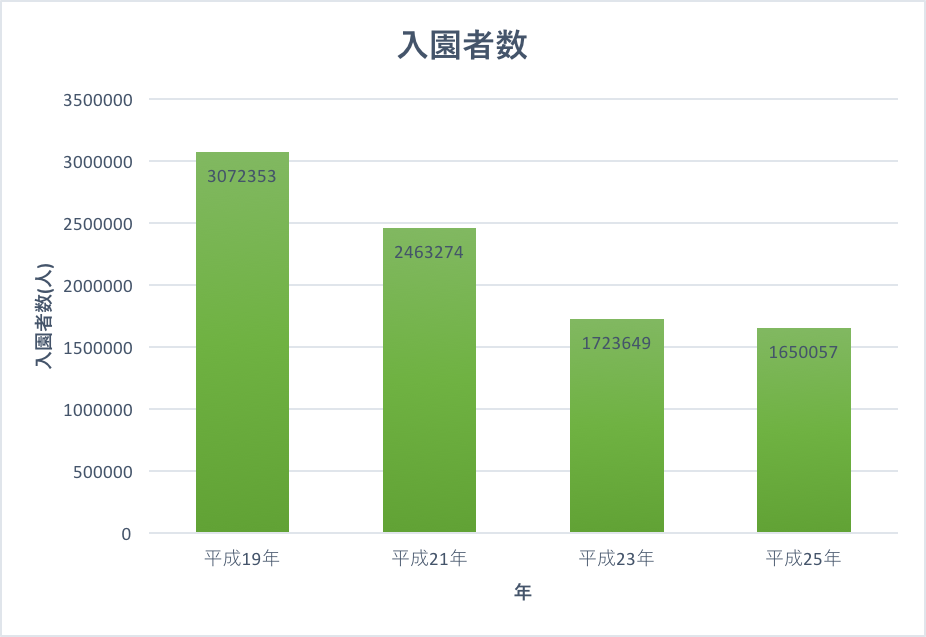
\includegraphics[width=0.5 \linewidth]{nyuensya.png}
		\caption{ある動物園の入園者数の遷移}
		\label{nyuensya}
	\end{center}
\end{figure}


\section{解決できる課題}
現在,多数の動物園で入園者数が減少し,更に大きな赤字が出ているという現状があります.このような問題が発生している原因として,
\begin{itemize}
	\item 他の動物園との差別化が行えていない
	\item 子供が楽しめるようなシステムが少ない
	\item 変化が少ないためリピーターが現れにくい
\end{itemize}
などが考えられます.

また,動物園は公立施設とされているため比較的安価である入園料の値上げも難しいという現状もあります.


\section{課題解決のための提案}
本提案書では上記の課題を解決するものとして「園内AR案内アプリ(仮)」を提案します.

本システムでは以下のような機能を提供します.

\begin{itemize}
	\item 動物の情報を表示する機能
	%カメラで写した動物の…を画面内に表示します
	\item スタンプラリー機能
	%あるオブジェクトをスタンプとし,カメラで写すことにより獲得できるようにします
	\item 言語表示切替機能
	%日本語,英語,中国語に切り替えることができるようにします
	\item 園内マップ機能
	%園内のマップを表示します.また,設定した場所までの案内を行います.
	\item お手洗いの混雑状況確認機能
	%お手洗いの使用状況を表示し,混雑を緩和します.
\end{itemize}


\section{課題解決のための方法}
このアプリケーションでは以下の装置を導入します.

\begin{itemize}
	\item スマートフォンのカメラを用いて動物情報,スタンプラリー,マップを表示するためのARアプリケーション
	\item お手洗いの使用状況を判断するためのWebカメラ
\end{itemize}

また,これらを管理するためのサーバの設置を行います.


\section{機能概要,前提条件,制約事項}

\subsection{機能概要}
\begin{enumerate}
	\item AR表示機能\\
	端末から動物を撮影することでその動物の詳細情報を画面上に表示します.画面には動物の名称を表示し,更にタップすることで詳細な説明画面へと遷移します.
	\item スタンプラリー機能\\
	指定したオブジェクトを画面に写すことでスタンプを獲得できるようにします.
	\item 言語表示切替機能\\
	アプリケーションに表示される文字を英語,中国語に対応させ,外国人観光客でも本システムを利用しやすくします.
	\item 園内マップ機能\\
	園内のマップを表示します.また,設定した場所までの案内を行います.
	\item 混雑状況確認機能\\
	カメラをトイレの入り口に設置します.また,撮影した静止画をサーバへと送信し,端末側から確認できるようにすることで混雑を緩和します.
	\item イベント通知機能\\
	動物園のイベント情報や新しい動物の情報などを通知します.
	%\item Liveカメラ機能\\
	%カメラを各動物が展示されている場所に設置します.本アプリケーションから動物のリアルタイムな映像を提供します.
\end{enumerate}

\subsection{前提条件}
本提案書では以下を前提条件としています.
\begin{itemize}
	\item 入場者が本システムの使用が可能な端末を所持していること
	\item 動物園がネットワーク環境下にあること
\end{itemize}

\subsection{制約事項}
本提案書では以下を制約条件としています.
\begin{itemize}
	\item 入場者が端末に本アプリケーションをインストールしていること
\end{itemize}

\section{情報の流れ}
このシステムは入力端末,利用端末,サーバ,Webカメラより構成します.システム内部での情報の流れを図~\ref{data_nagare}に示します.

\begin{figure}[H]
	\begin{center}
		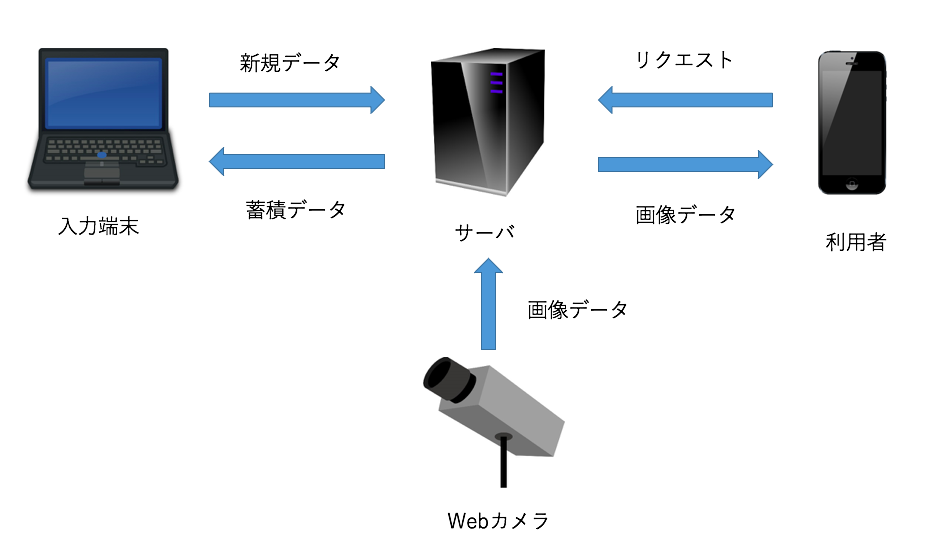
\includegraphics[width=0.8 \linewidth]{data_nagare.png}
		\caption{情報の流れ}
		\label{data_nagare}
	\end{center}
\end{figure}

利用者が撮影した画像をサーバに送信し,ARエンジンで画像認識を行う.認識して得た情報をもとに撮影した画像の情報を利用者端末に送信をする.

Webカメラで撮影した映像をサーバに送信し,サーバから利用者端末に送信する.

\section{システムインターフェース}
システム間のやりとりはHTTP通信を用いて行います.

\section{想定する利用者}
本システムを利用するものは以下の通りです.
\begin{itemize}
	\item 観光施設の従業員
	\item 観光施設の利用者
\end{itemize}

\section{システムのハードウェア構成,ソフトウェア構成}
システムのハードウェア構成は表\ref{hardware}の通りです.

\begin{table}[H]
	\caption{ハードウェア構成}
	\begin{center}
 		\begin{tabular}{|c|c|}\hline
			項目 & 数量 \\ \hline
			スマートフォン & 1台 \\ \hline
			サーバ用PC & 1台 \\ \hline
			Raspberry~Pi & 3台 \\ \hline
			Webカメラ & 3台\\ \hline
		\end{tabular}
		\label{hardware}
	\end{center}
\end{table}


ソフトウェアはwikitude,MySQL,javascript,HTML,CSSを用いて構成します.

\section{導入・移行計画}
2017年2月5日をもって,システムの導入を完了します.

\section{保守・運用}
提案システムを以下のように運用・保守します.

\begin{enumerate}
	\item 運用は管理者が行います.
	\item 故障発生時は弊社にて対応させていただきます.
\end{enumerate}

\section{作業標準}
システム開発にかかる作業標準は貴社ご指定のものを使用します.

\section{品質管理}
システム開発にかかる品質管理手法は貴社ご指定のものを使用します.

\section{工程計画}
工程計画は次の通りです.\\

要求分析完了:2017年10月26日

外部設計完了:2017年11月27日

内部設計完了:2017年12月18日

開発完了:2018年1月25日

導入:2018年2月5日

\section{体制}
このシステムの開発は弊社の9名のエンジニアにより実施します


\section{システム化にかかる費用とその効果}
システム化にかかる費用の概算は次の通りです.
\begin{table}[H]
  \caption{システム化にかかる費用}
  \begin{center}
    \begin{tabular}{|c|c|c|c|c|} \hline
      項目&単価(円)&数量&金額(円)&備考 \\ \hline
      Raspberry~pi&6,000&3台&18,000& \\ \hline
      USBカメラ&3,000&1台&3,000& \\ \hline
      サーバ用PC&150,000&1台&150,000& \\ \hline
      位置センサ&3,000&3台&9,000& \\ \hline
      保守・管理費& & & 減価償却期間& \\ \hline
      システム開発人件費&20,000&60日&&工数内訳 8人×60日 \\ \hline
      \multicolumn{3}{|c|}{合計}&& \\ \hline
    \end{tabular}
  \end{center}
\end{table}
システム化による効果の資産を以下に示します.前提条件として,入場者が本システムの使用が可能な端末を所持しており,動物園がネットワーク管理下にあると想定します.この場合,動物園来場者の増加,動物園来場者の満足度の向上などによるイメージアップが見込まれます.

利益と費用の比較

来場者は、宣伝や広告によってアプリをダウンロードし,アプリの機能を使用することで,野市動物園を効率よく楽しむことができます.

\section{本システム提案のアピールポイント}
本システム提案におけるアピールポイントについて説明します.
\begin{description}
\item[(1)] 動物園来場者に対して,動物園を効率的に楽しんで頂くためのAR搭載型アプリケーションシステムです.現在地や目的地をマップで表示することで,来場者の園内の移動効率を向上させます.
\item[(2)] 本アプリケーションは,英語,中国語に対応しているため,外国人来場者の方でも動物園をお楽しみ頂けます.
\item[(3)] 本アプリケーションでは,動物付近に設置されているwebカメラを中継し,園内の動物の様子を閲覧することができます.
\item[(4)] (1),(2),(3)のような多様な機能を実現させることによって,動物園の利用効率の向上を可能にさせます.その結果として来場者の増加や動物園のイメージアップが見込まれます.
\end{description}

\section{用語の定義}
  本提案書では、次の通りに用語を定義します.
  \begin{itemize}
  \item Raspberry~Pi: ARMプロセッサを搭載したシングルポートコンピュータ
    \item AR: Augmented~Reality(拡張現実)の略.現実世界の映像に対し,位置情報などのデータや実際に存在しない情報をCGと重ねて表示させる手法.
  \end{itemize}

\bibliographystyle{jplain}
\begin{thebibliography}{9}
\bibitem{ref1}
旭川市旭山動物園 年度別入園者数,\url{http://www5.city.asahikawa.hokkaido.jp/asahiyamazoo/zoo/siryou/nenbetu2014.pdf},2017年10月9日アクセス

\end{thebibliography}

\end{document}

